\label{sec:NuMUCCsel}

\par This chapter presents the two $\nu_{\mu}$ selections of the analysis. Both are inclusive selections, but with different distributions. The first selection (sec \ref{ssec:NuMUCCsel:INC}) provides a pure, high-statistics sample of $\nu_{\mu}$s and the second selection (sec \ref{ssec:NuMUCCsel:constr}) is optimized to be used as a constraining tool in the $\nu_e$ analysis. 

\subsubsection{Variable Definitions}
\label{sssec:NuMUCCsel:sel:vars}

\par \noindent \textbf{Slice variables}: These variables generally describe the reconstructed neutrino interaction, i.e. the confluence of data gathered from all the PFParticles in the slice.
\begin{itemize}
    \item \emph{nslice}: number of neutrino slices identified by the SliceID (possible values are 0 or 1).
    \item \emph{n\_tracks\_contained}: number of tracks fully contained in the fiducial volume.
    \item \emph{reco\_nu\_vtx\_sce\_\{x,y,z\}}: Reconstructed, spacecharge-corrected neutrino interaction vertices in (x,y,z) coordinates (see fig. \ref{fig:numu_vtx}.
    \item \emph{topological\_score}: A machine-learned quantity that reflects the complexity and directionality of observable slice quantities. This variable has strong discriminating power between signal and cosmic-background (see \ref{fig:numu_topo_pid} (possible values are between 0 and 1).
    \item \emph{CRT Veto and Distance Tagger}: Tools provided by the cosmic ray tagger (see sec. \ref{sec:sliceID:CRT}).
\end{itemize}

\par \noindent \textbf{Track variables}: These variables specifically describe the reconstructed PFParticles; in interest to this selection are reconstructed track-like objects. 
\begin{itemize}
    \item \emph{trk\_sce\_\{start,end\}\_\{x,y,z\}}: Reconstructed, spacecharge-corrected start/end-points for the tracks.
    \item \emph{trk\_llr\_pid\_score}: The log likelihood ratio particle identification score (see sec. \ref{subsec:loglikelihoodpid}). This variable has strong muon-proton discriminating power (see fig. \ref{fig:numu_topo_pid}).
    \item \emph{trk\_score}: A machine-learned quantity that describes how `track-like' the reconstructed object is (possible values between 0 and 1).
    \item \emph{trk\_len}: The length of the reconstructed track (in cm).
    \item \emph{trk\_distance}: The distance from the start-point of the reconstructed track to the reconstructed neutrino vertex (in cm).
    \item \emph{pfp\_generation}: The generation of the PFParticle according to Pandora, i.e. how many parents the object on interest has in the slice.
\end{itemize}

\subsubsection{Backgrounds}
\label{sssec:NuMUCCsel:sel:bkgrnds}

\par Coming soon...

\subsubsection{Fiducial Volume and Spacecharge-Corrected Spacepoints}
\label{sssec:NuMUCCsel:sel:FVandSCE}

\par Coming soon...

\begin{figure}
    \centering
    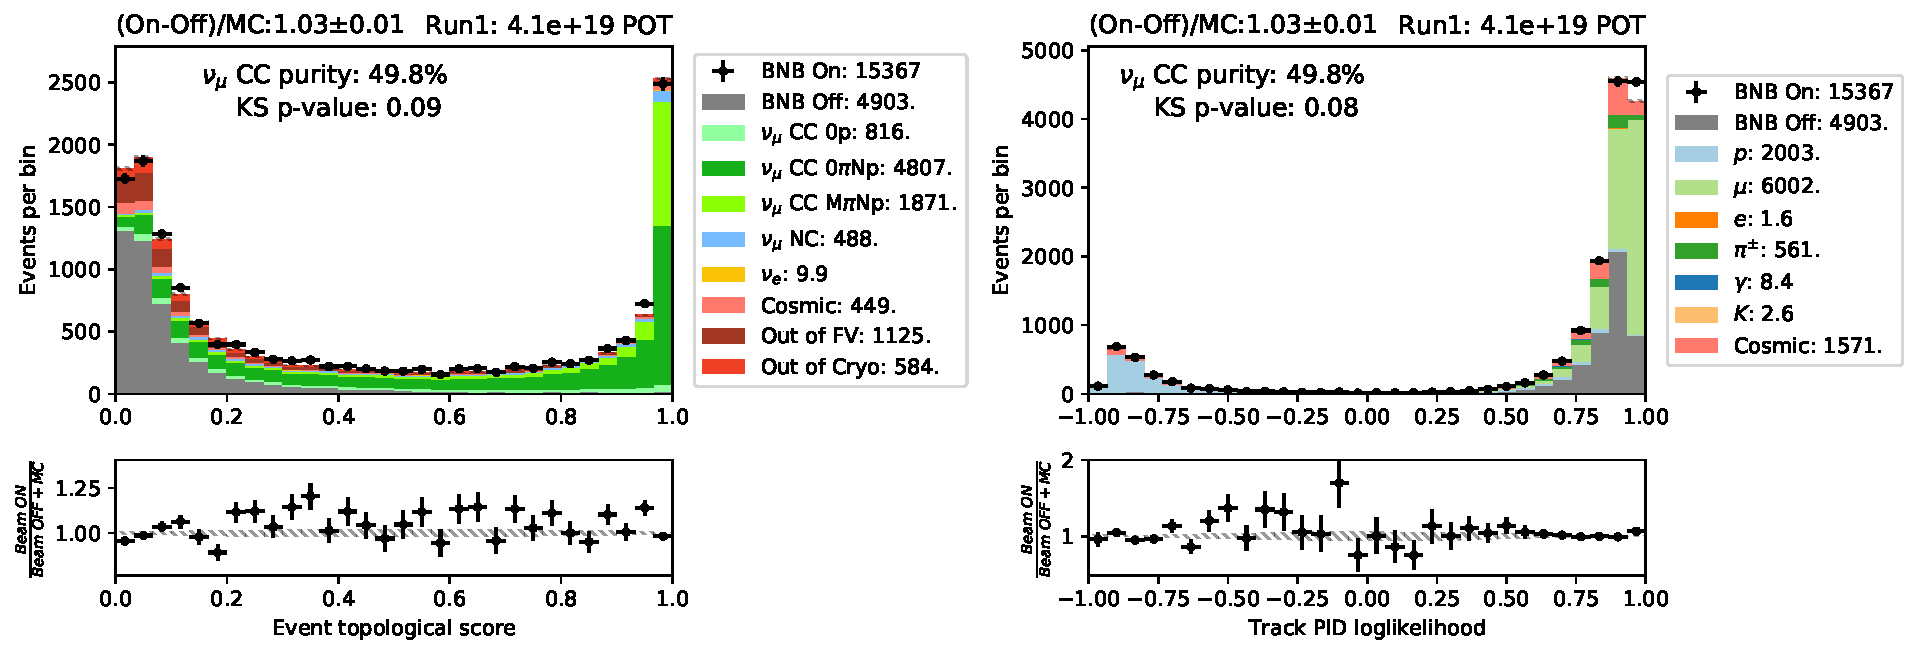
\includegraphics[width=\textwidth]{NuMuCCsel/Images/run1/numu_pret_run1.pdf}
    \caption{Caption}
    \label{fig:numu_topo_pid}
\end{figure}

\subsection{Inclusive Selection}
\label{ssec:NuMUCCsel:INC}

\subsubsection{Run 1}
\label{sssec:NuMUCCsel:INC:Run1}


\begin{figure}
    \centering
    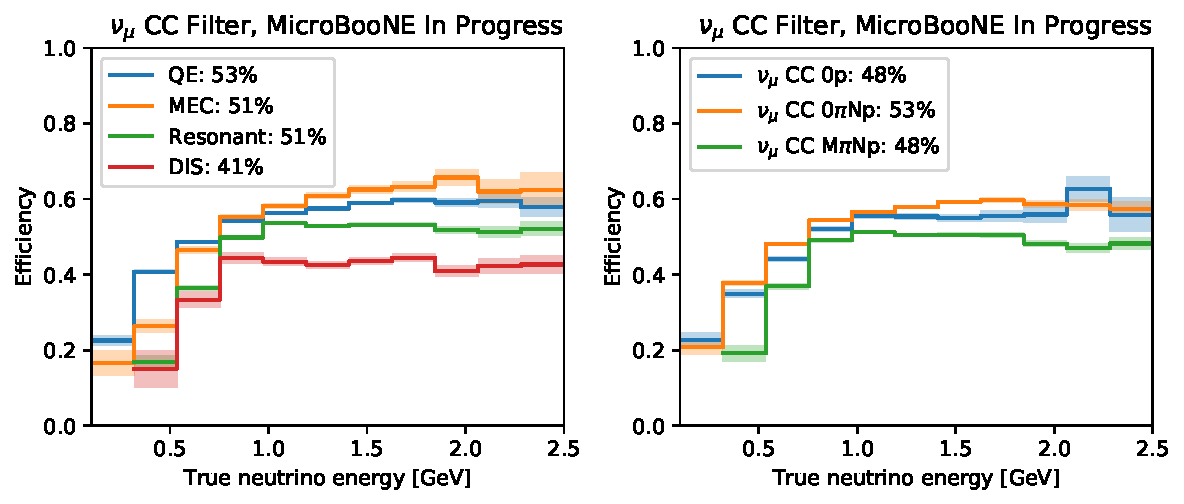
\includegraphics[width=0.85\textwidth]{NuMuCCsel/Images/run1/numu_efficiency_run1.pdf}
    \caption{Caption}
    \label{fig:numu_eff_r1}
\end{figure}

\begin{figure}
    \centering
    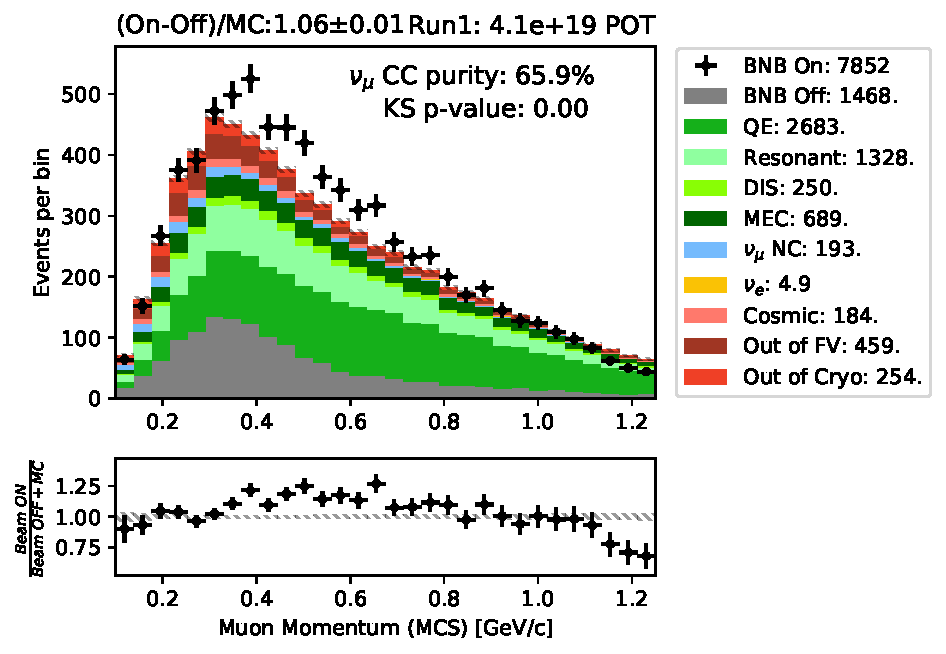
\includegraphics[width=0.495\textwidth]{NuMuCCsel/Images/run1/numu_mcsmom_run1.pdf} \hfill
    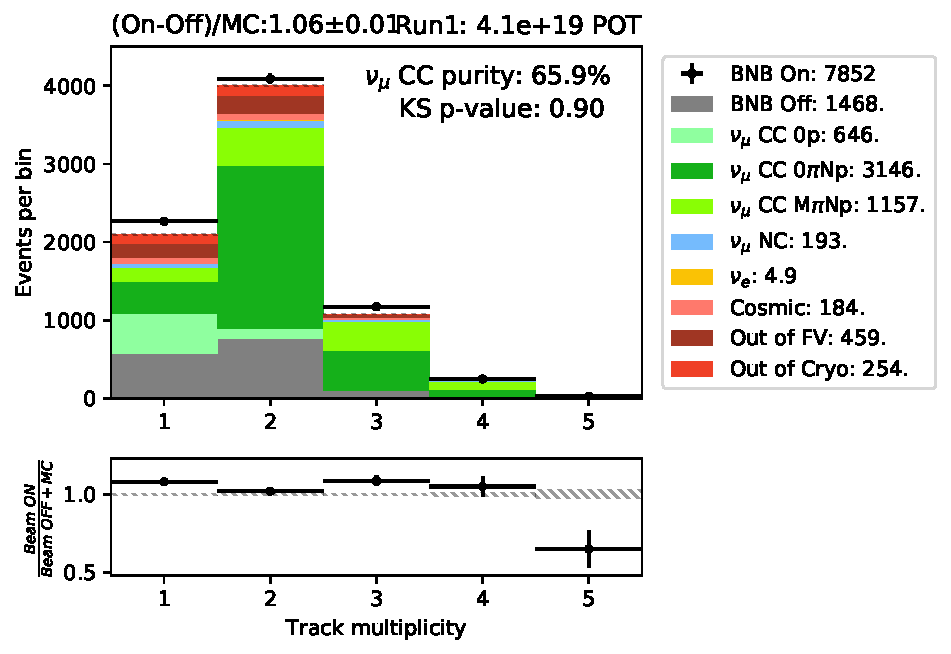
\includegraphics[width=0.495\textwidth]{NuMuCCsel/Images/run1/numu_vtxntrack_cat_run1.pdf}
    \caption{Caption}
    \label{fig:numu_mcs}
\end{figure}

\begin{figure}
    \centering
    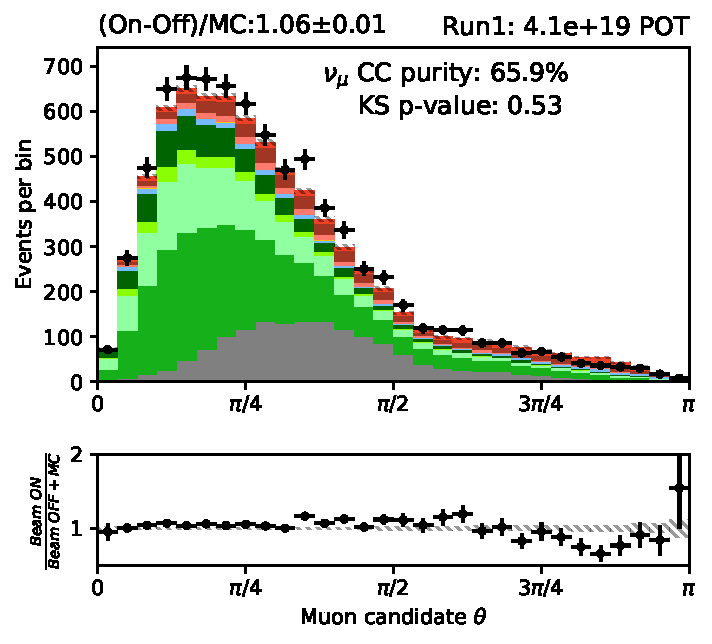
\includegraphics[height=6.5cm]{NuMuCCsel/Images/run1/numu_theta_run1.pdf} \hspace{2mm}
    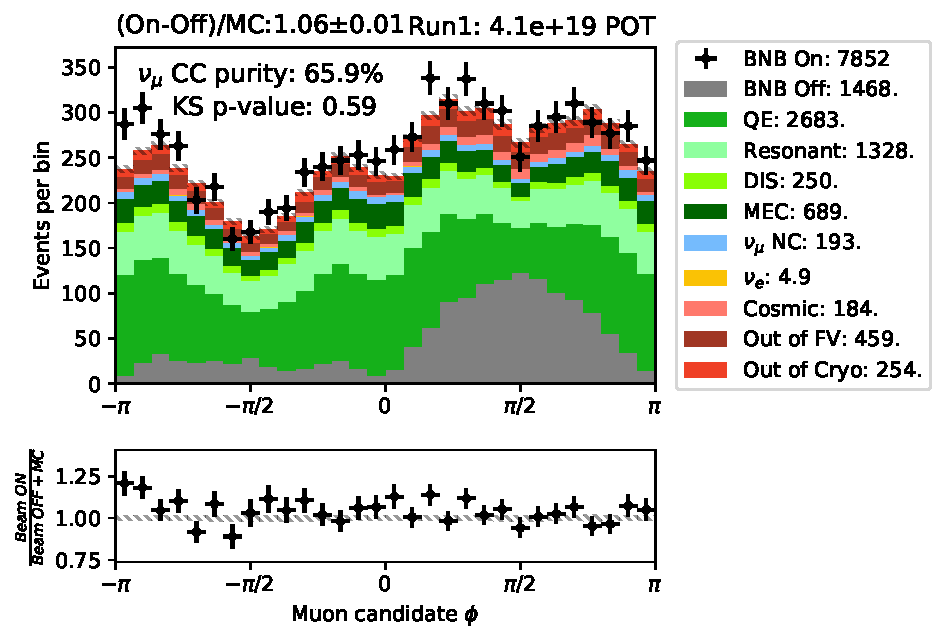
\includegraphics[height=6.5cm]{NuMuCCsel/Images/run1/numu_phi_run1.pdf}
    \caption{Caption}
    \label{fig:numu_angles}
\end{figure}

\begin{figure}
    \centering
    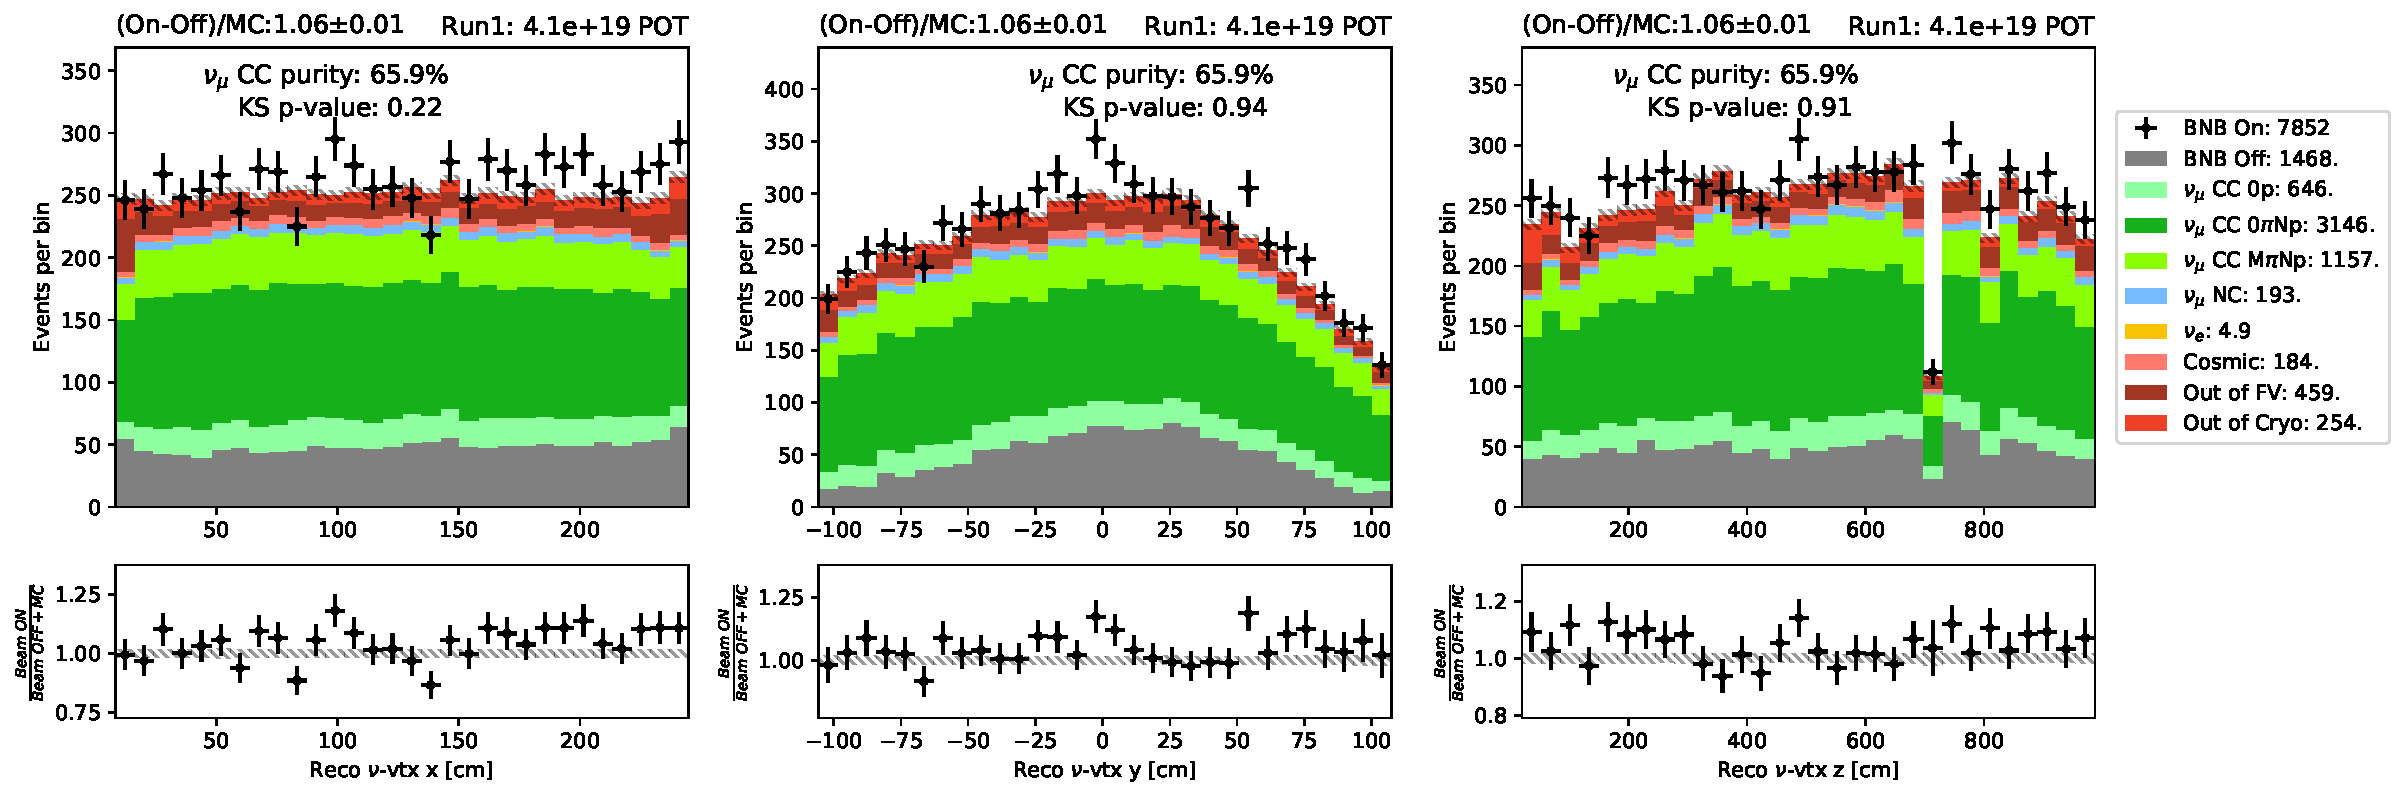
\includegraphics[width=\textwidth]{NuMuCCsel/Images/run1/numu_recovtx_run1.pdf}
    \caption{Caption}
    \label{fig:numu_vtx}
\end{figure}

\subsubsection{Run3}
\label{sssec:NuMUCCsel:INC:Run3}

\begin{figure}
    \centering
    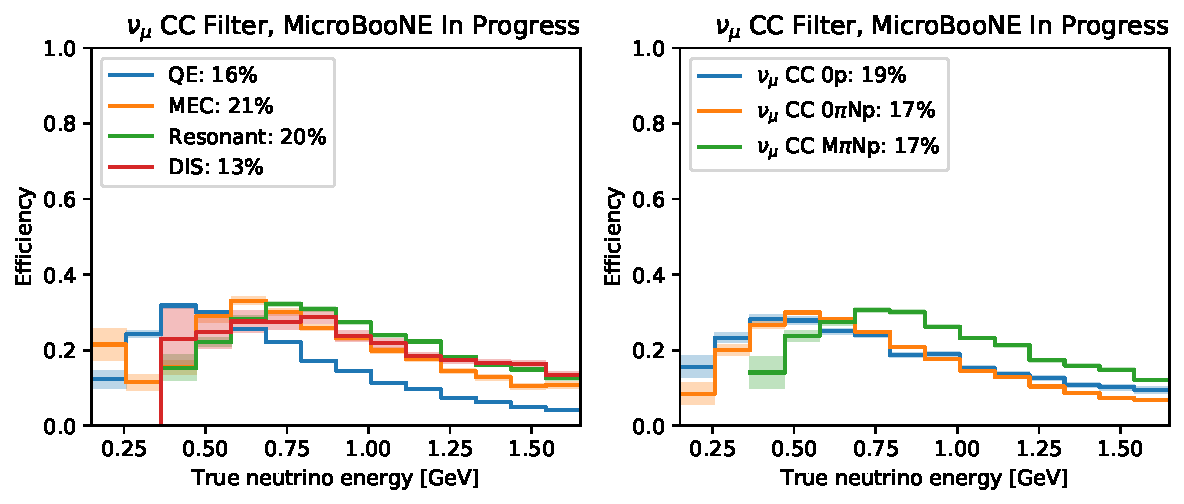
\includegraphics[width=0.85\textwidth]{NuMuCCsel/Images/run3/numu_efficiency_run3.pdf}
    \caption{Caption}
    \label{fig:numu_eff_r3}
\end{figure}


\begin{figure}
    \centering
    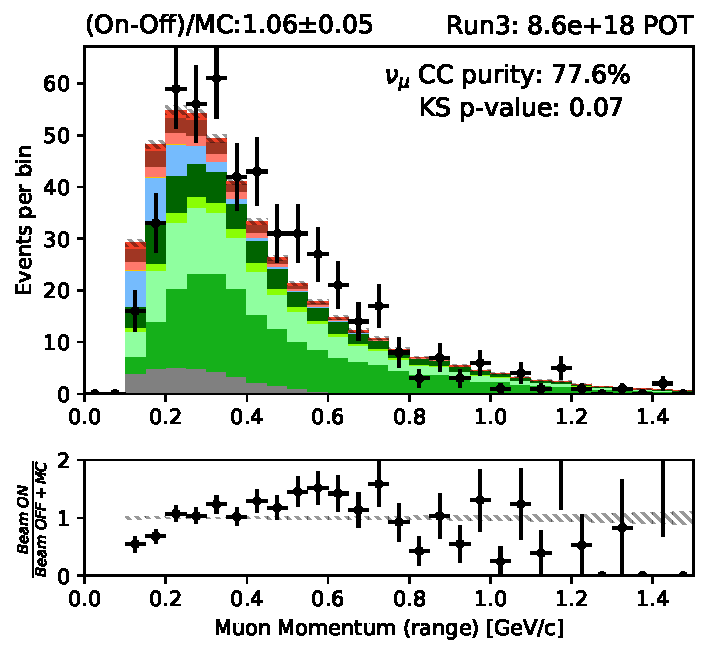
\includegraphics[height=6.5cm]{NuMuCCsel/Images/run3/numu_rangemom_run3.pdf} \hspace{2mm}
    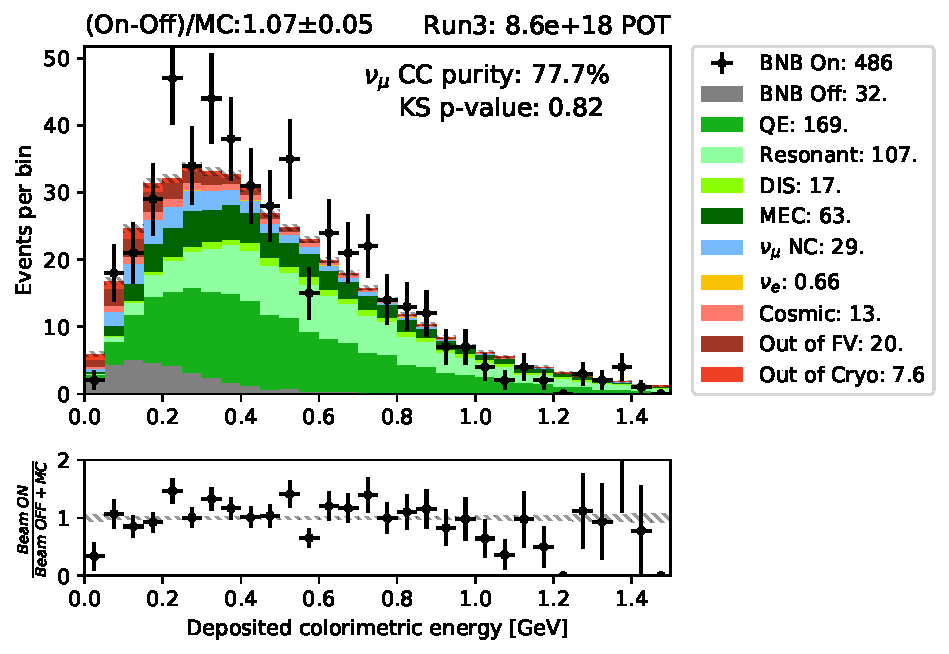
\includegraphics[height=6.5cm]{NuMuCCsel/Images/run3/numu_caloe_run3.pdf}
    \caption{Caption}
    \label{fig:numu_energy}
\end{figure}

\begin{figure}
    \centering
    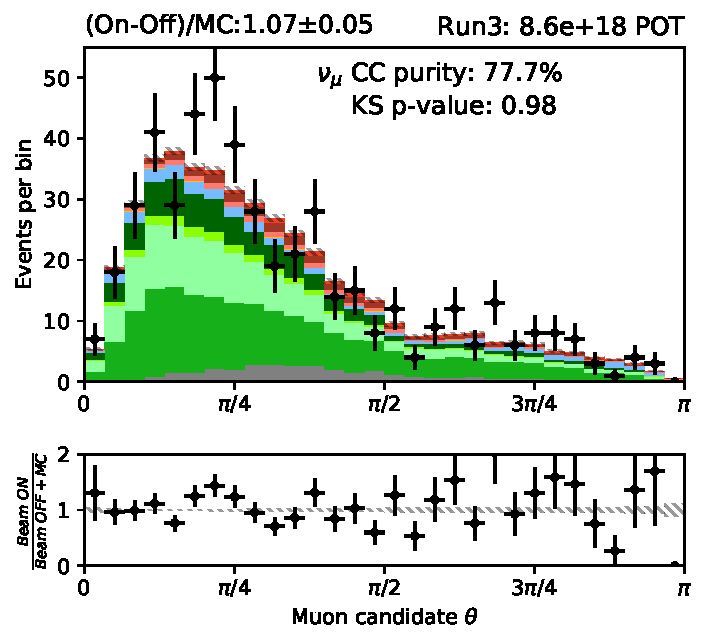
\includegraphics[height=6.5cm]{NuMuCCsel/Images/run3/numu_theta_run3.pdf} \hspace{2mm}
    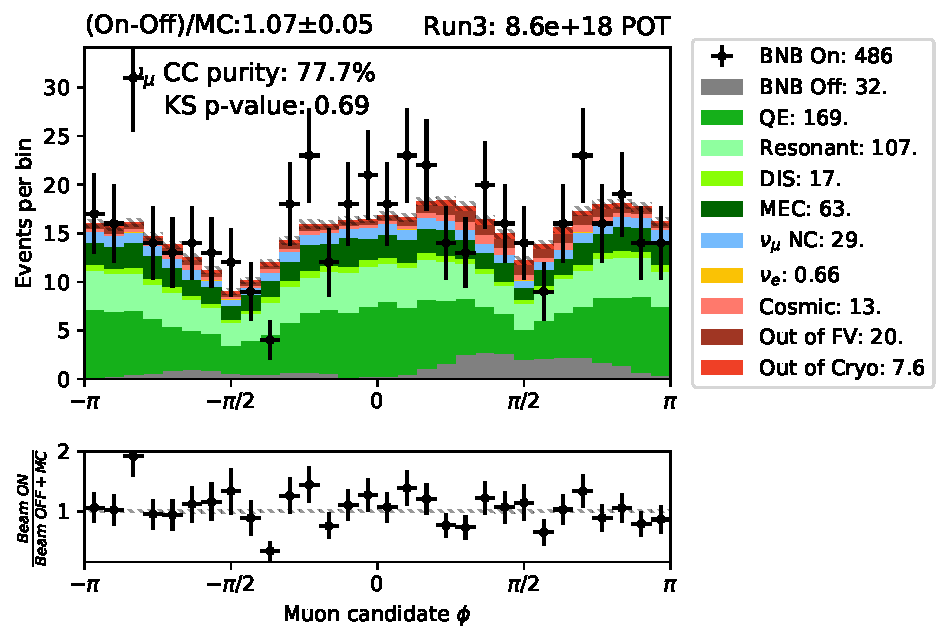
\includegraphics[height=6.5cm]{NuMuCCsel/Images/run3/numu_phi_run3.pdf}
    \caption{Caption}
    \label{fig:numu_angles}
\end{figure}

\subsection{$\nu_{\mu}$ Constraint \textcolor{red}{Ryan}}
\label{ssec:NuMUCCsel:constr}
\par The purpose of this $\nu_{\mu}$ side-band is to constrain the systematic uncertainties in the $\nu_{e}$ analysis. This is able to be done because the $\nu_{\mu}$s and $\nu_{e}$s of the BNB are subject to similar uncertainties, namely flux and cross-section modelling uncertainties. The $\nu_{e}$ selection is subject to higher uncertainties due to its low statistics. The $\nu_{\mu}$ component benefits from an order-of-magnitude advantage in absolute flux at MicroBooNE (Docdb 1031) and is exploited to constrain the uncertainties on the $\nu_{e}$s.

This selection prioritizes higher efficiencies in the lower-energy region that is the interest to the LEE analysis. The flux and cross-section $\nu_{e}$ are more uncertain in the few-hundreds MeV energy region. Fortunately, the absolute $\nu_{\mu}$ flux (fig \ref{fig:bnb_absoluteflux}) and the cross-species flux correlation is greatest below 1 GeV (figs \ref{fig:numuconstraint:flux}). 

\begin{figure}
    \centering
    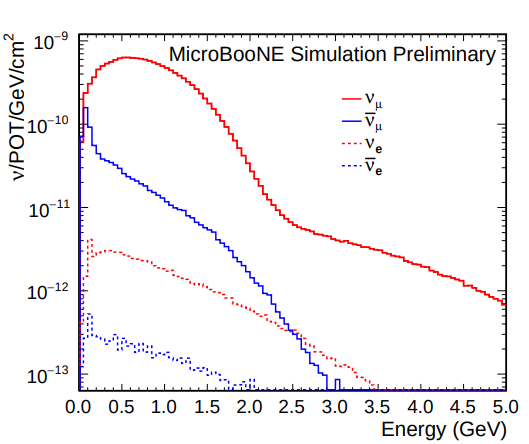
\includegraphics[height=6.5cm]{NuMuCCsel/Images/Ryan/absoluteFlux_uBooNE.png} \hspace{2mm}
    \caption{The absolute neutrino flux prediction through the MicroBooNE detector as calculated by the beam simulation. Shown is the flux for $\nu_{\mu}$, $\overline{\nu_{\mu}}$, $\nu_{e}$, and $\overline{\nu_{e}}$ averaged through the TPC volume with dimensions 2.56m×2.33m×10.37m. DocDb #1031}
    \label{fig:bnb_absoluteflux}
\end{figure}

\subsubsection{Signal Definition}
\label{sssec:NuMUCCsel:INC:signaldef}
\par A $\nu_{\mu}$ event is identified by the presence of, at least, one muon candidate originating from inside the fiducial volume of the detector. Additional tracks and showers may accompany the muon candidate; these assist in reconstruction but are not necessary in the inclusive selection.

\subsubsection{Event Selection and Muon Candidate Tagging}
\label{sssec:NuMUCCsel:sel}

\par The selection of $\nu_{\mu}$ events is built from the SliceID preselection (see sec. \ref{sec:sliceID:SliceID}) and a combination of cuts on slice-level and track-level observable values. The $\nu_{\mu}$ selection has this prescription: first, perform SliceID preselection; second, perform slice-level cuts to remove backgrounds; finally, perform track-level cuts to select one muon candidate.
\par Below is a summary of the variables used in this selection. There is some redundancy between this list and the lists given for the $\nu_e$ selection; this is intentional, as an overlap in phase space of the $\nu_{\mu}$ and $\nu_{e}$ selections improves constraining power.

\subsubsection{Event Selection}
\label{sssec:NuMUCCsel:sel:evt}

\par The cuts in this section are primarily designed to eliminate cosmic and dirt backgrounds and select slices that are $\nu_{\mu}$-like. The SliceID cut and the requirement of at least one reconstructed track are pursuant of $\nu_{\mu}$-like slices. The requirement that the reconstructed vertex be contained inside the fiducial volume and that the slice have a sufficiently high topological score favor $\nu_{\mu}$ CC events and disfavor activity that is cosmogenic or dirt-like. Those cuts, specifically, are:

\begin{itemize}
    \item \emph{nslice} = 1.
    \item \emph{n\_tracks\_contained} $>$= 1.
    \item \emph{reco\_nu\_vtx\_sce\_x} $\in$ [5,251] cm.
    \item \emph{reco\_nu\_vtx\_sce\_y} $\in$ [-110,110] cm.
    \item \emph{reco\_nu\_vtx\_sce\_z} $\in$ [20,986] cm.
    \item \emph{topological\_score} $>$ 0.06.
    \item \emph{reco\_nu\_vtx\_sce\_z} $\not\in$ [675,775] cm.
\end{itemize}

\par \noindent The final cuto on the $z$ coordinate is to ensure that it is not in the region of `dead wires' in the MicroBooNE detector. \textcolor{pink}{include some plot/statistic to motivate this further}

\par Run 3 has the additional power to leverage the CRT system to further limit cosmic contamination of the signal.

\textbf{Run 3 only:}
\begin{itemize}
    \item \emph{CRT Veto} != 1 or \emph{crthitpe} $<$ 100
    \item \emph{closestNuCosmicDist} $>$ 5 cm
\end{itemize}

\subsubsection{Muon Selection}
\label{sssec:NuMUCCsel:sel:muonsel}

\par After the slice-level cuts are applied, the tracks in the slice are further analyzed to identify a muon candidate.

\begin{itemize}
    \item \emph{trk\_sce\_start\_x} $\in$ [5,251] cm.
    \item \emph{trk\_sce\_start\_y} $\in$ [-110,110] cm.
    \item \emph{trk\_sce\_start\_z} $\in$ [20,986] cm.
    \item \emph{trk\_sce\_end\_x} $\in$ [5,251] cm.
    \item \emph{trk\_sce\_end\_y} $\in$ [-110,110] cm.
    \item \emph{trk\_sce\_end\_z} $\in$ [20,986] cm.
    \item \emph{trk\_llr\_pid\_score} $>$ 0.2.
    \item \emph{trk\_trk\_score} $>$ 0.8.
    \item \emph{trk\_trk\_length} $>$ 10 cm.
    \item \emph{trk\_trk\_distance} $<$ 4 cm.
    \item \emph{pfp\_generation} = 2.
\end{itemize}

\par \noindent The cuts made on the start and end points of the reconstructed tracks require that the track is fully contained inside the fiducial volume of the detector. This cut further limits the primary background for this selection which is cosmic muons, originating from outside the detector. The containment requirement also allows for the use of range-based momentum calculations on the muons; this has been shown to have a high resolution (see fig \ref{fig:numusel:momres}). The cut on the track distance requires that the reconstructed track be sufficiently close to the interaction vertex, this removes many in-time cosmics from the selection that are reconstructed as part of the slice. 
\par The cut on the log likelihood ratio pid score is to separate the muons from the protons among the PFParticle tracks in the passing slices. The track length cut further separates the muons from the protons which tend to have shorter track lengths. 

\par The track score cut ensures that the selected tracks are particularly track-like and this removes many particularly high energy, track-like electrons from the selection. Finally the PFParticle generation cut ensures that pandora recognizes that the track is a first daughter of the parent neutrino interaction. 


